% RESQ - PBL Phase 1 Report (3-page compressed)
\documentclass[10pt,a4paper]{article}

\usepackage[a4paper,left=1.5cm,right=1.5cm,top=1.35cm,bottom=1.2cm]{geometry}
\usepackage[T1]{fontenc}
\usepackage{lmodern}
\usepackage{graphicx}
\usepackage{xcolor}
\usepackage{array}
\usepackage{tabularx}
\usepackage{ragged2e}
\usepackage{enumitem}
\usepackage{fancyhdr}
\usepackage{tikz}
\usepackage{setspace}
\usetikzlibrary{positioning,arrows.meta,fit,backgrounds,calc}

\definecolor{TitleBlue}{RGB}{61,103,154}

\setlength{\parindent}{0pt}
\setlength{\parskip}{0pt}
\renewcommand{\arraystretch}{1.0}

\newcommand{\blueheading}[1]{{\sffamily\color{TitleBlue}\fontsize{12}{14}\selectfont #1}}
\newcommand{\bluebigheading}[1]{{\sffamily\bfseries\color{TitleBlue}\fontsize{13}{15}\selectfont #1}}

\newcommand{\abox}[1]{%
    \vspace{1.5pt}
    \noindent
    \fbox{%
        \begin{minipage}[t]{\dimexpr\textwidth-2\fboxsep-2\fboxrule\relax}
            \vspace{0.8mm}
            \itshape\fontsize{8.6}{10.4}\selectfont #1
            \vspace{0.8mm}
        \end{minipage}
    }
}

\pagestyle{fancy}
\fancyhf{}
\renewcommand{\headrulewidth}{0pt}
\renewcommand{\footrulewidth}{0pt}
\fancyhead[L]{\sffamily\bfseries\itshape\fontsize{9}{11}\selectfont PROBLEM BASED LEARNING (PBL) -- CSE (C / C++)}
\fancyhead[R]{\sffamily\bfseries\fontsize{9}{11}\selectfont PROJECT PROPOSAL}
\fancyfoot[R]{\itshape\fontsize{9}{11}\selectfont Page \thepage}
\setlength{\headheight}{12pt}
\setlength{\headsep}{10pt}
\setlength{\footskip}{14pt}

\newcommand{\memberrow}[8]{%
\begin{minipage}[t][5.35cm][t]{\linewidth}
\vspace{1mm}
\textbf{#1}
\end{minipage}
&
\begin{minipage}[t][5.35cm][t]{\linewidth}
\vspace{1mm}
\textit{#2 -- #3}\\
\textit{#4}\\
\textit{University Roll No.: #5}\\
\textit{Phone No.: #6}\\
\textit{Section: #8}
\end{minipage}
&
\begin{minipage}[t][5.35cm][t]{\linewidth}
\vspace{1mm}
\centering
\includegraphics[width=2.5cm,height=3.2cm]{#7}
\end{minipage}
\\
\hline
}

\begin{document}

\fontsize{9.5}{11.5}\selectfont

\bluebigheading{PROJECT AND TEAM INFORMATION}

\vspace{2.5mm}

\blueheading{Project Title}

\abox{RESQ --- Intelligent Disaster Rescue \& Emergency Response Simulator. \textbf{``Algorithms That Save Lives.''}}

\vspace{3mm}

\blueheading{Student / Team Information}

\vspace{1.5mm}

\noindent
{\fontsize{10}{13}\selectfont
\begin{tabularx}{\textwidth}{|>{\RaggedRight\arraybackslash}p{0.26\textwidth}|>{\RaggedRight\arraybackslash}X|>{\Centering\arraybackslash}p{2.9cm}|}
\hline
\begin{minipage}[t]{\linewidth}
\vspace{1mm}
\textit{Team Name / Team \#}
\vspace{1mm}
\end{minipage}
&
\begin{minipage}[t]{\linewidth}
\vspace{1mm}
\textit{RESQ Force} \quad --- \quad \textbf{Team ID: DSCPP-III-2026-T117}
\vspace{1mm}
\end{minipage}
&
\begin{minipage}[t]{\linewidth}
\vspace{1mm}
\textit{Photo}
\vspace{1mm}
\end{minipage}
\\
\hline
\memberrow{Team member 1 (Team Lead)}{Vanya Rathi}{2510383410}{2510383410@geu.ac.in}{2028514}{9259011570}{member1.jpg}{DS-2}
\memberrow{Team member 2}{Akshat Dobhal}{2510370353}{2510370353@geu.ac.in}{2028631}{9389135760}{member2.jpg}{ML-2}
\memberrow{Team member 3}{Ayush Kandwal}{2510380235}{2510380235@geu.ac.in}{2028405}{9068120181}{member3.jpg}{ML-4}
\memberrow{Team member 4}{Nitin Singh}{2510370229}{2510370229@geu.ac.in}{2028786}{6395245688}{member4.jpg}{ML-1}
\end{tabularx}}

\vspace{1.5mm}

\noindent\textit{\textbf{Project Mentor:} Mr. Prabhdeep Singh} \hfill \textit{\textbf{Team ID:} DSCPP-III-2026-T117}

\newpage

\bluebigheading{PROPOSAL DESCRIPTION}

\vspace{2.5mm}

\blueheading{Motivation}

\abox{When an earthquake, a flood, a fire or a highway pile-up happens, the calls come in much faster than the number of teams, ambulances and hospital beds that are actually free. In those first few hours the operator has to decide, on a phone line, who gets help first. There is no single screen showing how badly each victim is hurt, which team is idle, or which road is still open. Two teams end up at the same spot, a serious case waits behind a minor one, and an ambulance drives into a street that collapsed an hour ago.\\[0.8mm]
If we look at it as programmers, this is really a computing problem. Sorting requests by urgency, giving out limited resources and finding the fastest path on a broken road network are exactly the jobs that priority queues, graphs, Dijkstra's algorithm, BFS, stacks and linked lists are meant for. That is where the idea for RESQ came from. We wanted something small enough to run offline on any college lab machine, without internet or paid GIS software, that a control room or a mock drill could use to test dispatch decisions and to show, with numbers, that priority-based dispatch beats plain first-come-first-served.}


\vspace{3mm}

\blueheading{State of the Art / Current Solution}

\abox{In India most emergency help today goes through the 112 and 108 call centres. An operator notes down the call and sends the nearest free ambulance. The order is mostly the order in which calls arrive, and how urgent a case is depends on the operator's own judgement. Bigger agencies buy Computer-Aided Dispatch software such as Hexagon or Motorola PremierOne, and use ArcGIS or Google Maps for routing. On the ground, triage is done on paper using the START or SALT colour tags.\\[0.8mm]
Each of these has a weak point. The commercial CAD suites are costly, closed and need a working network, so they are of little use exactly when towers and links go down. Map APIs assume the roads are fine, so they cannot know about a collapsed bridge or a flooded lane. Paper triage tags help the person standing there, but they never become a list a computer can re-order across all pending victims. Most college and research prototypes we read about solve either triage or routing, not both together. RESQ tries to put the two in one free, offline C/C++ program that also keeps a record of every decision it made.}


\vspace{3mm}

\blueheading{Project Goals and Milestones}

\abox{\textbf{General goals.} We want to build a menu-driven C/C++ simulator that keeps the disaster area as a graph of locations, takes in rescue requests, sorts victims by how serious their condition is using a priority queue, hands out rescue teams, ambulances and hospital beds, finds the shortest route with Dijkstra's algorithm, stores every operation on a stack so it can be undone or replayed, and finally prints statistics such as average response time, number of victims rescued and how busy each resource was. The last step is to run the same scenario with plain first-come-first-served dispatch and compare the two.\\[0.8mm]
\textbf{Milestones.}
\begin{itemize}[leftmargin=5mm,topsep=0.4mm,itemsep=0.2mm]
\item \textbf{M1 (Week 1--2):} Requirement study, class diagram, module split; C structures for Victim and Location; linked-list victim registry.
\item \textbf{M2 (Week 3):} Queue for normal requests and priority queue (min-heap on severity, tie-broken by arrival time) for critical victims.
\item \textbf{M3 (Week 4):} Graph module --- adjacency list of the disaster map, BFS area exploration, Dijkstra shortest-route engine.
\item \textbf{M4 (Week 5):} C++ OOP layer --- Victim, RescueTeam, Ambulance, Hospital, Disaster, Location, RescueOperation classes with inheritance and polymorphism.
\item \textbf{M5 (Week 6):} Allocation logic, stack-based operation history with undo, sorting and searching of victims and resources.
\item \textbf{M6 (Week 7):} File persistence, statistics and comparison report, console dashboard.
\item \textbf{M7 (Week 8):} Testing with three scenarios (earthquake, flood, fire), documentation and final demonstration.
\end{itemize}}

\vspace{3mm}

\blueheading{Project Approach and Technologies}

\abox{RESQ is written in two layers. The \textbf{C layer} holds the plain data structures and algorithms, and the \textbf{C++ layer} sits on top of it and turns them into an object-oriented simulation.\\[0.8mm]
\textbf{C --- Data Structures \& Algorithms.} Victim and rescue records are kept in linked lists, so records can be added or removed while the simulation is running. Ordinary requests wait in a normal FIFO queue. Critical victims go into a priority queue built as a binary min-heap, ordered by a severity score from 1 (critical) to 5 (minor), with arrival time breaking ties so nobody is starved. Every completed operation is pushed on a stack, which gives us replay and undo almost for free. The disaster area itself is a weighted graph stored as an adjacency list. Nodes are places like shelters, hospitals and collapsed buildings, and each edge weight is the travel time on that road; a blocked road simply gets an infinite weight. BFS tells us which zones are still reachable, and Dijkstra gives the shortest path from the team's base to the victim and then on to the nearest hospital. Merge sort and quick sort are used to rank victims and resources, and binary or linear search pulls a record out by its ID.\\[0.8mm]
\textbf{C++ --- OOP design.} An abstract class \textit{Person} is inherited by \textit{Victim} and \textit{RescueTeam}. \textit{Ambulance} and \textit{RescueTeam} both come from a common \textit{Resource} base that declares a virtual \texttt{dispatch()} method, so the engine can call the same function on any unit and the right version runs. \textit{Hospital}, \textit{Location}, \textit{Disaster} and \textit{RescueOperation} keep their data private and expose it through member functions, and constructors and destructors take care of allocating and freeing memory.\\[0.8mm]
\textbf{Platform \& tools.} C11 and C++17 built with GCC/G++ on MinGW and Linux, VS Code and Code::Blocks as editors, Git and GitHub for version control, and a Makefile so each module builds separately. Maps, victims and logs are stored as plain \texttt{.txt} and \texttt{.csv} files, diagrams are drawn in draw.io, and the output is shown on a coloured console dashboard. For testing we write our own disaster scenarios and also check boundary cases such as an empty queue or a fully cut-off sector.}

\newpage

\blueheading{System Architecture (High Level Diagram)}

\vspace{1.5pt}
\noindent
\fbox{%
\begin{minipage}[t]{\dimexpr\textwidth-2\fboxsep-2\fboxrule\relax}
\centering
\vspace{1.5mm}
\begin{tikzpicture}[
  scale=0.85, transform shape,
  font=\sffamily\tiny,
  box/.style={draw=TitleBlue!80,fill=TitleBlue!8,rounded corners=2pt,align=center,inner sep=2pt,minimum height=6mm,text width=26mm},
  ar/.style={-{Latex[length=1.4mm]},draw=TitleBlue!70}
]
\node[box] (ui) {Console UI / Dashboard\\ \textit{menu, reports}};
\node[box,right=16mm of ui] (ctrl) {Simulation Controller\\ \textit{(C++ engine loop)}};
\node[box,below=5mm of ui] (intake) {Request Intake\\ \textit{Queue (normal)}};
\node[box,below=5mm of ctrl] (triage) {Triage Module\\ \textit{Priority Queue (critical)}};
\node[box,below=5mm of intake] (alloc) {Resource Allocator\\ \textit{RescueTeam, Ambulance, Hospital}};
\node[box,below=5mm of triage] (route) {Routing Engine\\ \textit{Graph + BFS + Dijkstra}};
\node[box,below=5mm of alloc] (records) {Records Store\\ \textit{Linked List (victims)}};
\node[box,below=5mm of route] (hist) {Operation History\\ \textit{Stack (undo/replay)}};
\node[box,below=5mm of $(records)!0.5!(hist)$,xshift=0mm] (files) {File Persistence\\ \textit{map.txt, victims.csv, log.txt}};
\draw[ar] (ui) -- (ctrl);
\draw[ar] (ctrl) -- (triage);
\draw[ar] (ctrl) -- (intake);
\draw[ar] (intake) -- (alloc);
\draw[ar] (triage) -- (route);
\draw[ar] (triage) -- (alloc);
\draw[ar] (alloc) -- (route);
\draw[ar] (alloc) -- (records);
\draw[ar] (route) -- (hist);
\draw[ar] (records) -- (files);
\draw[ar] (hist) -- (files);
\end{tikzpicture}

\vspace{1mm}
{\itshape\tiny C layer: Queue, Priority Queue, Linked List, Stack, Graph, BFS, Dijkstra, Sort/Search \quad$|$\quad C++ layer: Victim, RescueTeam, Ambulance, Hospital, Disaster, Location, RescueOperation}
\vspace{1mm}
\end{minipage}}

\vspace{4mm}

\blueheading{Project Outcome / Deliverables}

\abox{\begin{itemize}[leftmargin=5mm,topsep=0.4mm,itemsep=0.4mm]
\item A working menu-driven RESQ simulator in C and C++, compiled with GCC, that registers victims, sorts them by severity, gives out rescue teams, ambulances and hospital beds, and prints the shortest rescue route.
\item Source code kept in separate modules so each one can be reused: linked list, queue, priority queue (min-heap), stack, graph with BFS and Dijkstra, sorting and searching, plus the C++ classes.
\item Three ready-to-run scenarios (earthquake, flood and fire) with sample map and victim files, so the demo does not need fresh typing every time.
\item A statistics module and a short comparison report that puts priority-based dispatch next to first-come-first-served dispatch on average response time, victims rescued and resource use.
\item Log files of the rescue history and the operation stack, so the run can be checked afterwards.
\item Documentation: class diagram, architecture diagram, a table of time complexities, a user manual and a README on GitHub.
\item A final presentation with a live run of one complete rescue cycle.
\end{itemize}}

\vspace{4mm}

\blueheading{Assumptions}

\abox{We assume the disaster map is given as an input file and does not change on its own; roads only open or close when the simulation triggers an event. Each victim already carries a severity number from 1 to 5, the way a first responder would tag them on the spot. Travel time is taken as proportional to the edge weight, so traffic and weather are left out. The number of rescue teams, ambulances and hospital beds is fixed when the run starts, and one ambulance handles one victim at a time. All data is either typed in or read from files, since we have no live GPS or sensor feed. Finally, the program is meant for a single user on a single machine.}

\vspace{4mm}

\blueheading{References}

\abox{\begin{enumerate}[leftmargin=6mm,topsep=0.4mm,itemsep=0.3mm]
\item Cormen, Leiserson, Rivest \& Stein, \textit{Introduction to Algorithms}, 4th ed., MIT Press --- priority queues, BFS, Dijkstra's algorithm.
\item Bjarne Stroustrup, \textit{The C++ Programming Language}, 4th ed. --- OOP, inheritance and polymorphism.
\item Kernighan \& Ritchie, \textit{The C Programming Language}, 2nd ed. --- pointers, structures, dynamic memory.
\item National Disaster Management Authority (NDMA), India --- Guidelines on Medical Preparedness and Mass Casualty Management. \texttt{https://ndma.gov.in}
\item START / SALT mass-casualty triage protocols, U.S. Dept. of Health \& Human Services. \texttt{https://chemm.hhs.gov/startadult.htm}
\item GeeksforGeeks --- Graph representations, Dijkstra and heap implementations. \texttt{https://www.geeksforgeeks.org}
\item E. W. Dijkstra, ``A note on two problems in connexion with graphs,'' \textit{Numerische Mathematik}, 1959.
\item Emergency Response Support System (ERSS-112), Ministry of Home Affairs, India. \texttt{https://112.gov.in}
\end{enumerate}}

\end{document}
